\documentclass[]{article}
\usepackage{lmodern}
\usepackage{amssymb,amsmath}
\usepackage{ifxetex,ifluatex}
\usepackage{fixltx2e} % provides \textsubscript
\ifnum 0\ifxetex 1\fi\ifluatex 1\fi=0 % if pdftex
  \usepackage[T1]{fontenc}
  \usepackage[utf8]{inputenc}
\else % if luatex or xelatex
  \ifxetex
    \usepackage{mathspec}
  \else
    \usepackage{fontspec}
  \fi
  \defaultfontfeatures{Ligatures=TeX,Scale=MatchLowercase}
\fi
% use upquote if available, for straight quotes in verbatim environments
\IfFileExists{upquote.sty}{\usepackage{upquote}}{}
% use microtype if available
\IfFileExists{microtype.sty}{%
\usepackage{microtype}
\UseMicrotypeSet[protrusion]{basicmath} % disable protrusion for tt fonts
}{}
\usepackage[margin=1in]{geometry}
\usepackage{hyperref}
\hypersetup{unicode=true,
            pdftitle={Target-based site prioritization under climate change using quadratic network flow},
            pdfauthor={Derek Corcoran},
            pdfborder={0 0 0},
            breaklinks=true}
\urlstyle{same}  % don't use monospace font for urls
\usepackage{longtable,booktabs}
\usepackage{graphicx,grffile}
\makeatletter
\def\maxwidth{\ifdim\Gin@nat@width>\linewidth\linewidth\else\Gin@nat@width\fi}
\def\maxheight{\ifdim\Gin@nat@height>\textheight\textheight\else\Gin@nat@height\fi}
\makeatother
% Scale images if necessary, so that they will not overflow the page
% margins by default, and it is still possible to overwrite the defaults
% using explicit options in \includegraphics[width, height, ...]{}
\setkeys{Gin}{width=\maxwidth,height=\maxheight,keepaspectratio}
\IfFileExists{parskip.sty}{%
\usepackage{parskip}
}{% else
\setlength{\parindent}{0pt}
\setlength{\parskip}{6pt plus 2pt minus 1pt}
}
\setlength{\emergencystretch}{3em}  % prevent overfull lines
\providecommand{\tightlist}{%
  \setlength{\itemsep}{0pt}\setlength{\parskip}{0pt}}
\setcounter{secnumdepth}{5}
% Redefines (sub)paragraphs to behave more like sections
\ifx\paragraph\undefined\else
\let\oldparagraph\paragraph
\renewcommand{\paragraph}[1]{\oldparagraph{#1}\mbox{}}
\fi
\ifx\subparagraph\undefined\else
\let\oldsubparagraph\subparagraph
\renewcommand{\subparagraph}[1]{\oldsubparagraph{#1}\mbox{}}
\fi

%%% Use protect on footnotes to avoid problems with footnotes in titles
\let\rmarkdownfootnote\footnote%
\def\footnote{\protect\rmarkdownfootnote}

%%% Change title format to be more compact
\usepackage{titling}

% Create subtitle command for use in maketitle
\providecommand{\subtitle}[1]{
  \posttitle{
    \begin{center}\large#1\end{center}
    }
}

\setlength{\droptitle}{-2em}

  \title{Target-based site prioritization under climate change using quadratic network flow}
    \pretitle{\vspace{\droptitle}\centering\huge}
  \posttitle{\par}
    \author{Derek Corcoran}
    \preauthor{\centering\large\emph}
  \postauthor{\par}
    \date{}
    \predate{}\postdate{}
  
\usepackage{booktabs}
\usepackage{longtable}
\usepackage{array}
\usepackage{multirow}
\usepackage{wrapfig}
\usepackage{float}
\usepackage{colortbl}
\usepackage{pdflscape}
\usepackage{tabu}
\usepackage{threeparttable}
\usepackage{threeparttablex}
\usepackage[normalem]{ulem}
\usepackage{makecell}
\usepackage{xcolor}

\begin{document}
\maketitle

\hypertarget{introduction}{%
\section{Introduction}\label{introduction}}

Currently, 14.9\% of terrestrial area is a part of the global protected area network (UNEP-WCMC 2018). However, most of this areas have not been created using priorization tools developed to maximize species or ecosystems conservation based on current biodiersity patterns (Rodrigues et al. 2004; Jenkins et al. 2015). The situation is even worst when we take into account that the range of species will change over time (Araújo et al. 2004; Chen et al. 2011; Lenoir et al. 2008; Regos et al. 2016), were several species that are now being protected by these areas might not be protected in the future because of the climate crisis (Alagador, Cerdeira, and Araújo 2014; Araújo et al. 2004).

Despite the concern about protected area planning, a review Jones et al. (2016) shows that more than 90\% of the priorization planing studies that try to incorporate climate change, only take two time steps into account, current climate and the last step of climate. Currently, two of the most used tools for conservation planning are Prioritizr and Zonation (Di Minin et al. 2014; Hanson et al. 2019). Zonation can be used for conservation prioritization under climate change as conservation features may be explicitly linked through interaction. This allows for simultaneous prioritization of a species current range, its modeled future range, and the connectivity between the two limited by a species' capacity to disperse.

\begin{table}[H]
\centering
\begin{tabular}{lllll}
\toprule
 & Network flow & Zonation & Migclim & Prioritizr\\
\midrule
Considers more than 2 time-slices & Yes & No & Yes & No\\
Can add species to the solutions afterwards & Yes & No & Yes & No\\
Keep track of species dispersal routes & Yes & Yes & Yes & No\\
Solves for conservartion targets & Yes & Yes & No & Yes\\
Considers cost as part of the solution & Yes & Yes & No & Yes\\
\bottomrule
\end{tabular}
\end{table}

However, in order for the species to move from areas were they are currently protected to the future protected areas, their route has to be protected as well, that is the biological corridors that they will use (Nuñez et al. 2013; Rosenberg, Noon, and Meslow 1997). Thus, the planification and creation of those biological corridors correspond to adaptative measures to environmental changes that would mitigate the impacts of the climate crisis (Hannah et al. 2007). In that context, biological corridors should consider effects of climate crisis, changes in land use and habitat fragmentation, in order to evaluate the factibility of the species reaching future available habitat.

There have been several approaches trying to model biological corridors. Local approaches have focus just in one or a few species (Alagador, Cerdeira, and Araújo 2014; Cushman et al. 2013; Gregory et al. 2014) or group of species (Beier, Majka, and Bayless 2007; Phillips et al. 2008; Williams et al. 2005), not being able to be use for planning for lack of species or be in confined spaces, respectibly. A continental approach was made by Lawler et al. (2013), who modeled biological corridors in the Americas. Even when that model was made for close to 3,000 species did not consider species dispersal speed or use the information to build priority areas. Among these articles, the work of Phillips et al. (2008), incorporates the use of the Network Flow optimization method (Ahuja, Magnanti, and Orlin 1993) in order to solve the problem expressed by Williams et al. (2005), generating a solution 33\% more efficient than previous optimization methods. This makes this methodology one of the most promising ways of solving conservation planning problems through the use of biological corridors.

In its traditional use, Network flow gives the best possible solution given constrains (Phillips et al. 2008). If we looked at the solution for a species in a raster, every cell would have a value of either one or zero, where one would be a cell necesary for the conservation of the species or a zero if it is not necessary. This best solution, however, only represents one of the possible solutions to conserve a species, and does not give us any alternatives. in this research we present Quadratic Cost Network Flow as alternative solution, where for every species we would still get a value of one if the cell is irrepleacable for the solution, zero if that cell is not needed, and an intermediate value for cells that are one of many alternative solutions for a given species, this is, for every cell we have an irreplaceability index. Spatial planning is a complex endeavour where agendas and/or needs evolve rapidly and several alternative subopitmal solutions might be needed in order to navigate this complex decisions.

In this article we present a new method of working with network flow on conservation planning using quadratic costs, while at the same time comparing its results and implications with traditional network flow and zonation, using the Northern Tropical Andes ecorregion as an example.

\hypertarget{methods}{%
\section{Methods}\label{methods}}

\hypertarget{area}{%
\subsection{Area}\label{area}}

The studied area was the Northern Tropical Andes, consisting of the countries of Colombia, Venezuela and Ecuador, with a buffer of 200 kilometers arround land areas.

\begin{figure}

{\centering 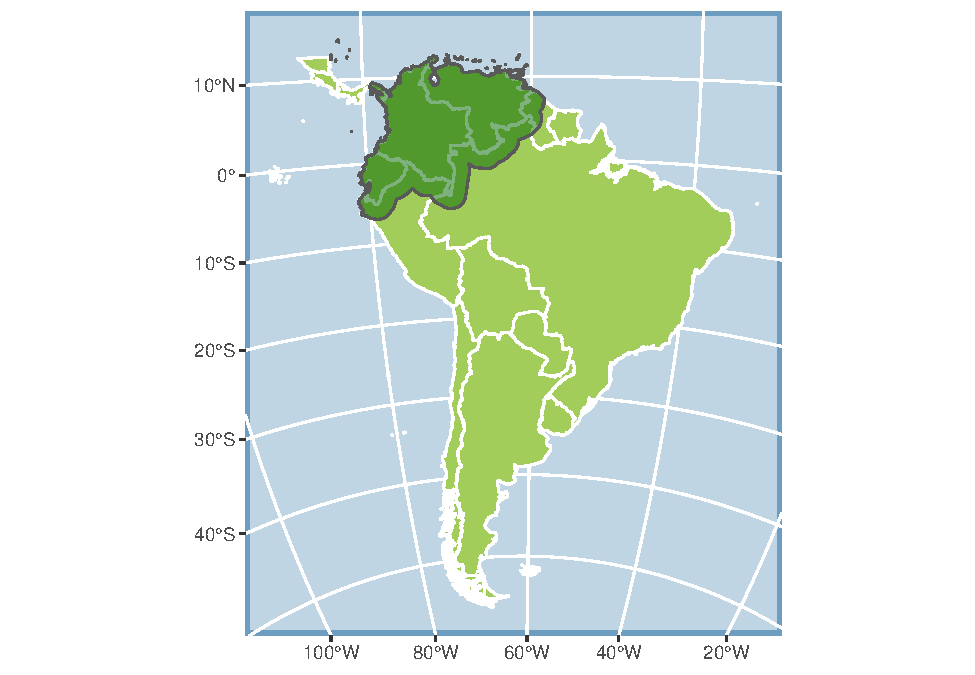
\includegraphics{NFPaper_files/figure-latex/MapArea-1} 

}

\caption{Map of Southamerica, the darkened area is the area where the priorization was performed}\label{fig:MapArea}
\end{figure}

The studied area is shown in figure \ref{fig:MapArea} and it encompases 3,632,762 square kilometers

\hypertarget{species}{%
\subsection{Species}\label{species}}

671 species of plants were used for the model, only endemic species were used in this study. A list can be found in the supplementary materials

\hypertarget{gcms}{%
\subsection{GCMs}\label{gcms}}

First GCMComparer was used in order to select the 4 GCMs as shown in figure \ref{fig:Diagrama}, then R was used to generate distribution models for each GCM using the Dismo Package. Then each model was projected as a binary response (presence-absense) for all decades form 2000 (present) to 2070 completing 8 time slices for each species.

For each Species, a network of dispersion into each timeslice was generated using the QuadCostAmpl package, and finally we solved for Network Flow using the AMPL software using the Gurobi solver

\begin{figure}
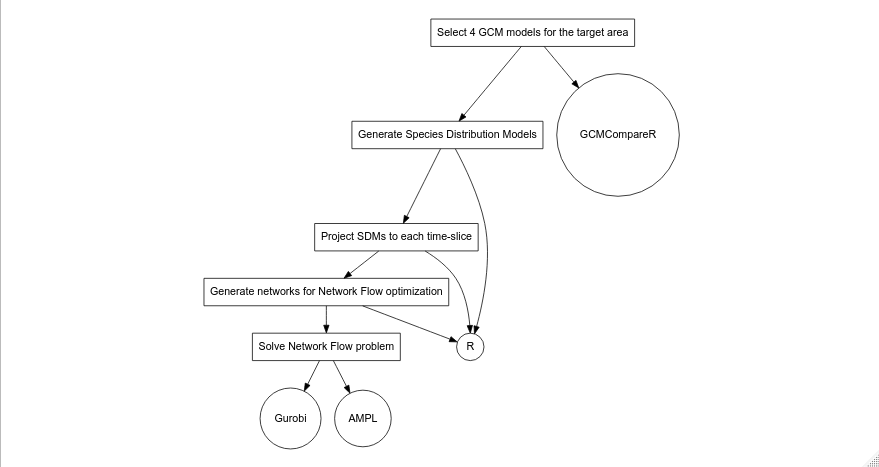
\includegraphics[width=4.39in]{Diag1} \caption{All the steps and programs used in the Optimization}\label{fig:Diagrama}
\end{figure}

Four GCM models were selected to project the species distribution using the GCMcompareR shiny app (Fajardo et al. 2018), we followed the storylines approach (Zappa and Shepherd 2017) and selected a GCM warmer and wetter, warmer and dryier, colder and wetter, and colder and dryier than the ensemble. The selected models where cc, cn, la, mp al the process is shonw in in figure \ref{fig:Diagrama}.

\hypertarget{niche-modeling}{%
\subsection{Niche modeling}\label{niche-modeling}}

For each species the species distribution model was fit using the dismo package (Hijmans et al. 2017), using 50,000 random background points and the maxent algorithm (Phillips, Anderson, and Schapire 2006; Merow, Smith, and Silander Jr 2013)

\hypertarget{model-description}{%
\subsection{Model Description}\label{model-description}}

This model was developed based on the notion of non-overlapping dispersal chains (Williams et al. 2005), and instead of having a binary solution (to protect or not protect an area), the result will be an index of importance going from zero to one. Here, zero means that there are no chains passing by that spacial point that go from the source to the final destination, and one is a point where chains have to pass through to reach the desired flow.
In order to do this, we follow Network-flow methods (Ahuja, Magnanti, and Orlin 1993) to model the survival and dispersion of species along the space and time, using species distribution models and quadratic flow costs to split the flow evenly across alternative paths. Therefore, the resulting flow across an arc is high only if there are few alternatives to use that edge to achieve the target flow.
Even when model takes into account protected areas (cost zero) and human habitat such as cities (cost infinite) in the decision making, both were not included in this exercise to simplify the examples. This is a generalist model which only needs the distribution model of the species projected to each time slice and the maximum dispersal distance for each species.

\hypertarget{model-formulation}{%
\subsubsection{Model Formulation}\label{model-formulation}}

The objective is to minimize the cost

\(\underset{Quadcost}{\text{minimize}}\)

\[\small Quadcost =  \sum_{i=1}^n{(Cost\times Flow_t)^2}\]

\(\text{subject to}\)

\[\small \text{Initial Flow} = \sum_{i=1}^n{Flow_{t_1}} = \text{Target paths}\]

\[\small \text{Final Flow} = \sum_{i=1}^n{Flow_{t_{final}}} = \text{Target paths}\]

\[\small \text{Flow capacity} = \sum_{i=1}^n{Flow_{(i,t)}} \leq capacity_{(i,t)}\]

\hypertarget{network-generation}{%
\subsection{Network generation}\label{network-generation}}

Ir order to generate the networks de QuadCostAmpl package was used (Corcoran and Fajardo 2019)

\hypertarget{linear-network-flow}{%
\subsection{Linear Network FLow}\label{linear-network-flow}}

Model

\hypertarget{quadratic-network-flow}{%
\subsection{Quadratic Network Flow}\label{quadratic-network-flow}}

\hypertarget{zonation}{%
\subsection{Zonation}\label{zonation}}

\emph{In the examples above, (a) uses the Present Simple tense to
describe what is normally done or to describe a standard piece of equipment
used in the research and (b) uses the Past Simple tense to describe what
you did yourself.}

\emph{Another diffi culty arises with the passive when you write about the
procedure you used and compare it with the work of other researchers.
You can use the Past Simple agentless passive to describe the procedure
you used (the samples were collected using a suction tube) but you may
also need to use exactly the same Past Simple agentless passive to describe
the procedure used by the other researcher whose work you are citing (the
samples were collected using a suction tube).}

\emph{One way to make sure that your own contribution is clear and easy
to identify is by marking it with words --- perhaps by adding phrases
like} \textbf{In this study}, \emph{the samples were collected using a suction tube or} \textbf{In
our experiments} \emph{the samples were collected using a suction tube, and by
identifying the procedure used by other researchers with careful references
at the appropriate place in the sente}

\hypertarget{results}{%
\section*{Results}\label{results}}
\addcontentsline{toc}{section}{Results}

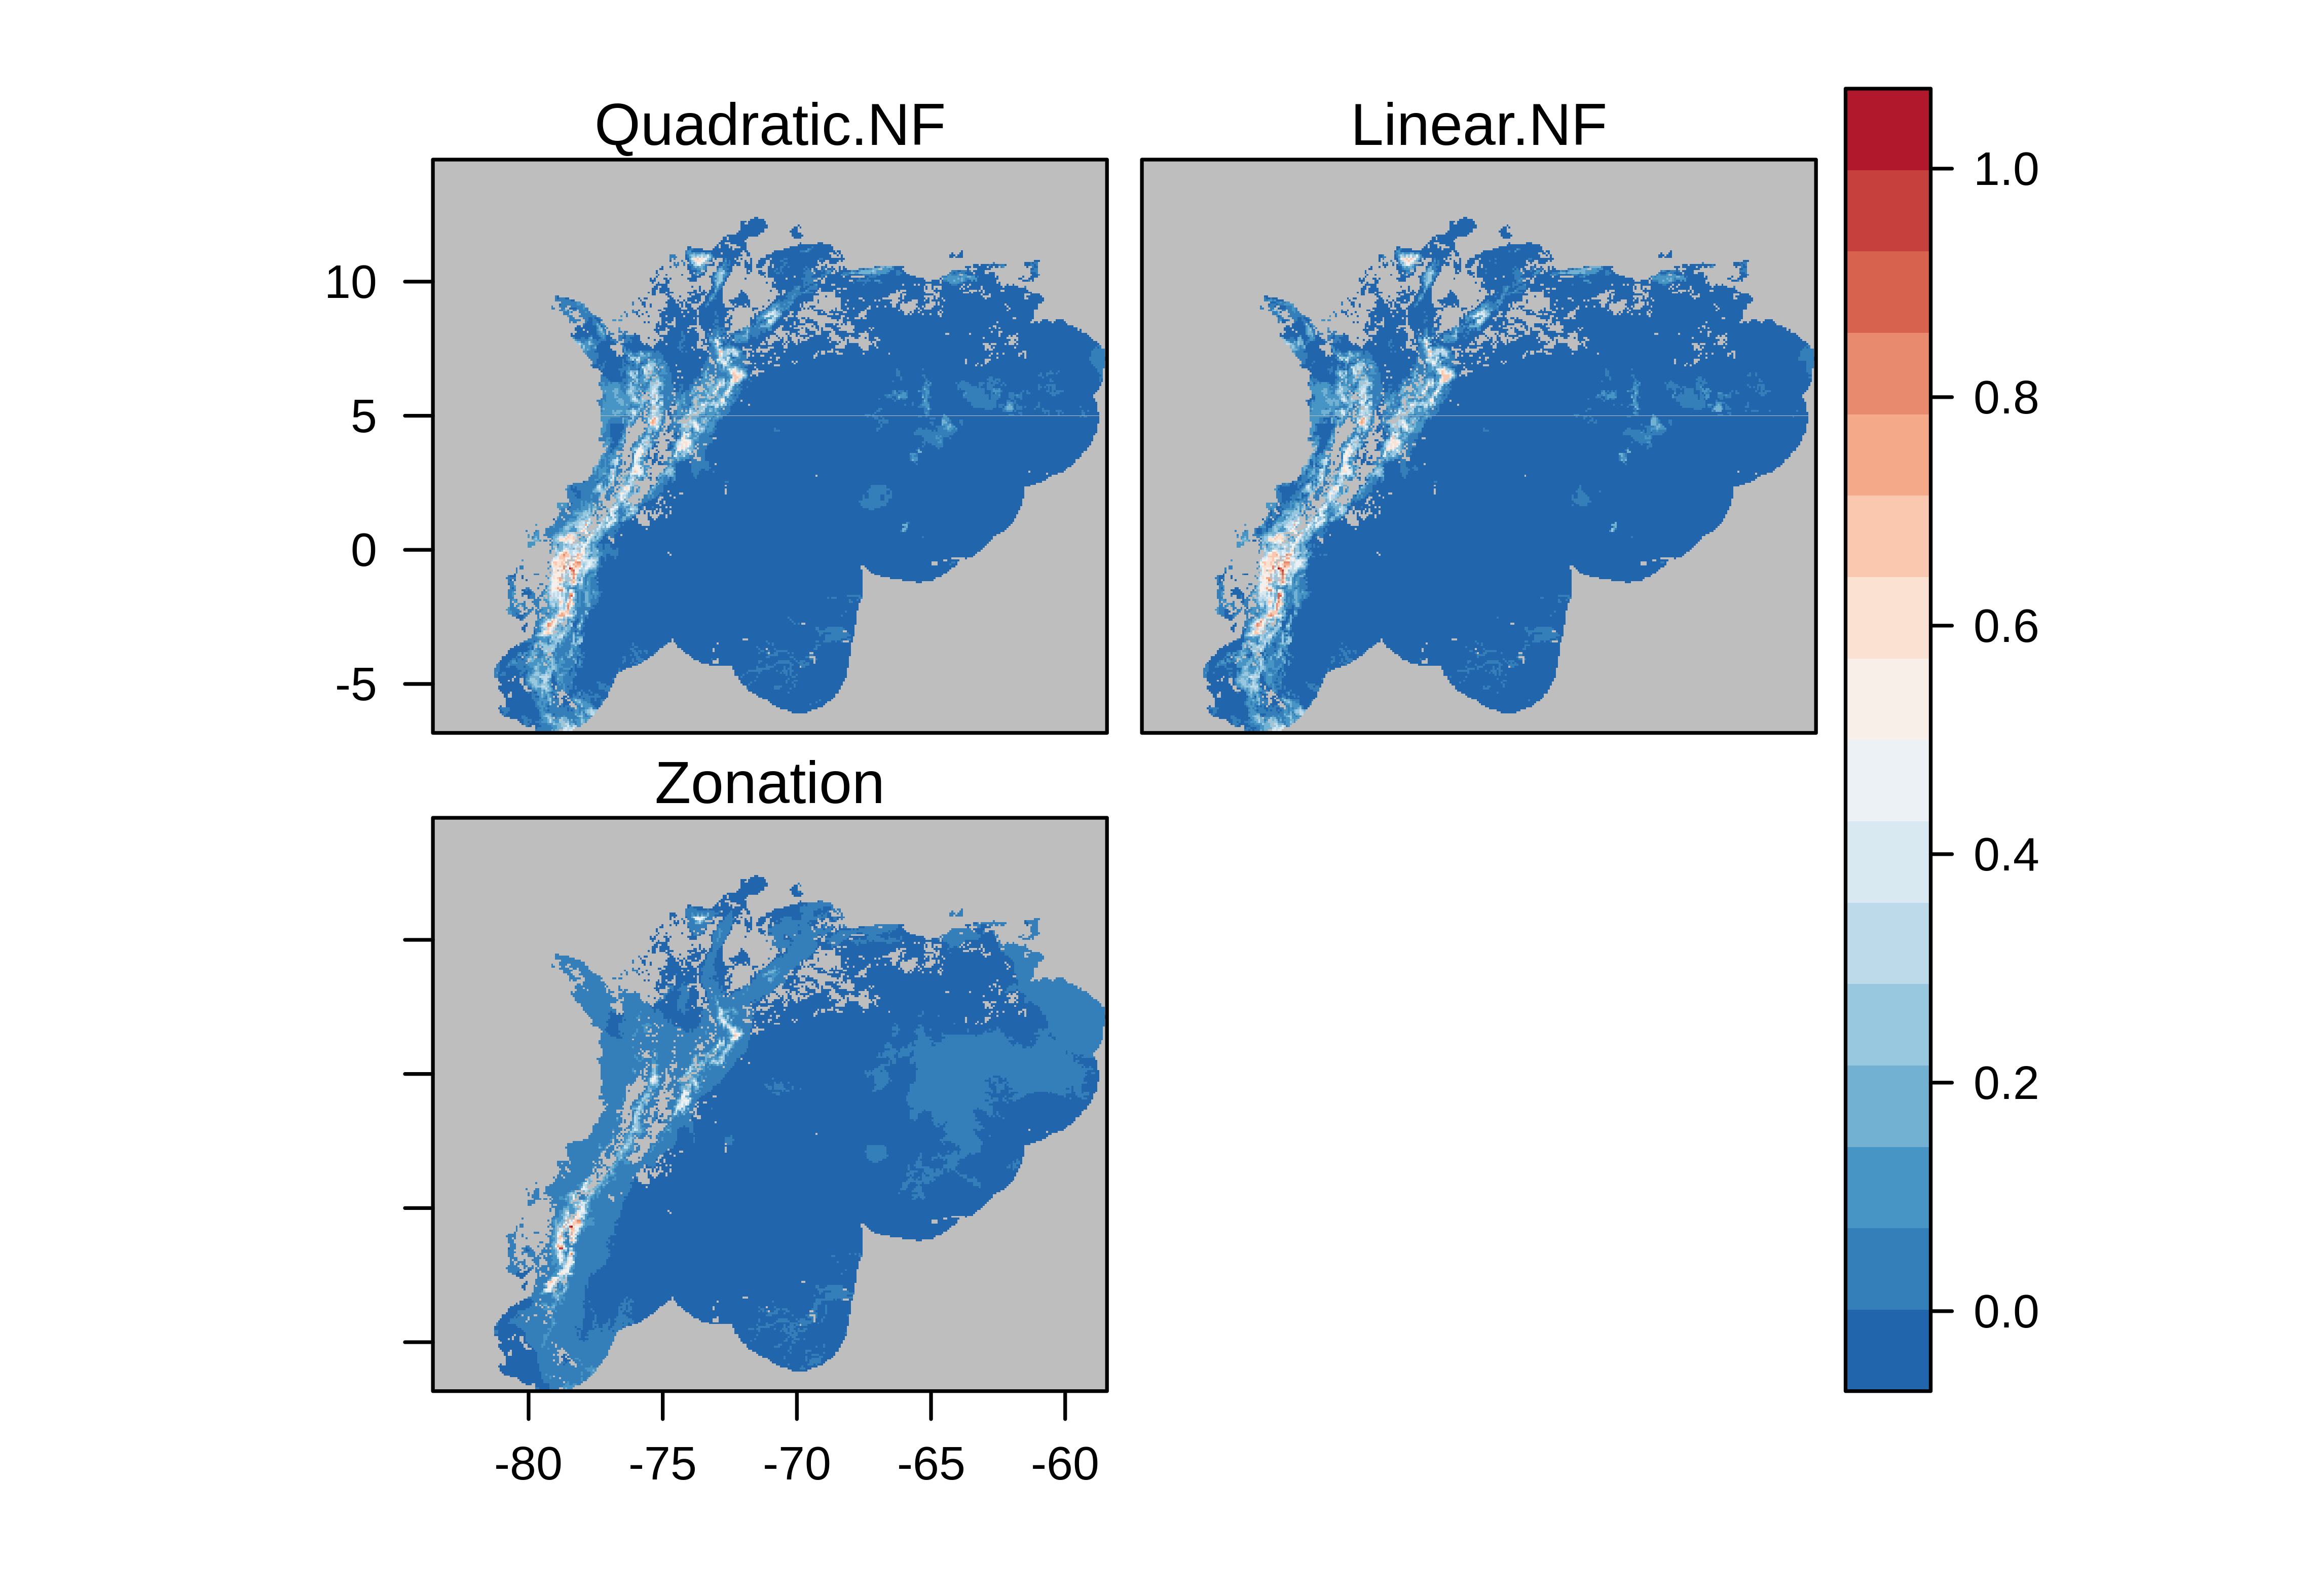
\includegraphics{NFPaper_files/figure-latex/AllSols-1.png}

\begin{itemize}
\tightlist
\item
  \textbf{For methods:} Since one of the main objectives of prorization methods is to rank the cells within an area, we used Spearman's rho correlation, that estimates the rank-based measure of association. We also calculated a local Spearman correlation on a matrix of five by five cells, in order to figure out if there are zome important
\end{itemize}

The results of all three algorithms is shonw in figure \ref{fig:AllSols}, at first glance, the thre algorithms havee very similar results, however, when we look at the Spearman correlation of all three methods we start seeing some important differences, where Quadratic and Linear Network flow have a spearman correlation of 0.92, but both methods have a smaller correlation with zonation, with Quadratic Network Flow having a higher correlation of 0.669, vs linear network flow having a correlation of 0.624 with Zonation. When we look at the local correlation plots (figure \ref{fig:LocalCorr}), we see that for the most part, the local correlations are all mostly possitive, specially between both Network Flow algorithms. There are some blue areas in the figure, when comparing those priorities with zonation. Representing some big discrepancies in local priorization, that is mostly localized

when we look at the boxplot of local correlation values (figure \ref{fig:Boxplot}), we see that the lower whiskers in the comparizon of both NetworkFlow methods with Zonation, are bellow zero

\begin{itemize}
\tightlist
\item
  \textbf{For discusion:} One of the main problems at comparing Network Flow vs Zonation, is that Zonation will give a rank to each and every cell in the study area, which is not true for Network Flow. It comes as no surprise that Quadratic Network flow has a higher correlation with Zonation than Linear Network flow, the intended result of quadratic network flow being more similar to zonation than linear network flow.
\end{itemize}

\hypertarget{efficiency-comparison-number-of-cells}{%
\subsubsection{Efficiency comparison (Number of cells)}\label{efficiency-comparison-number-of-cells}}

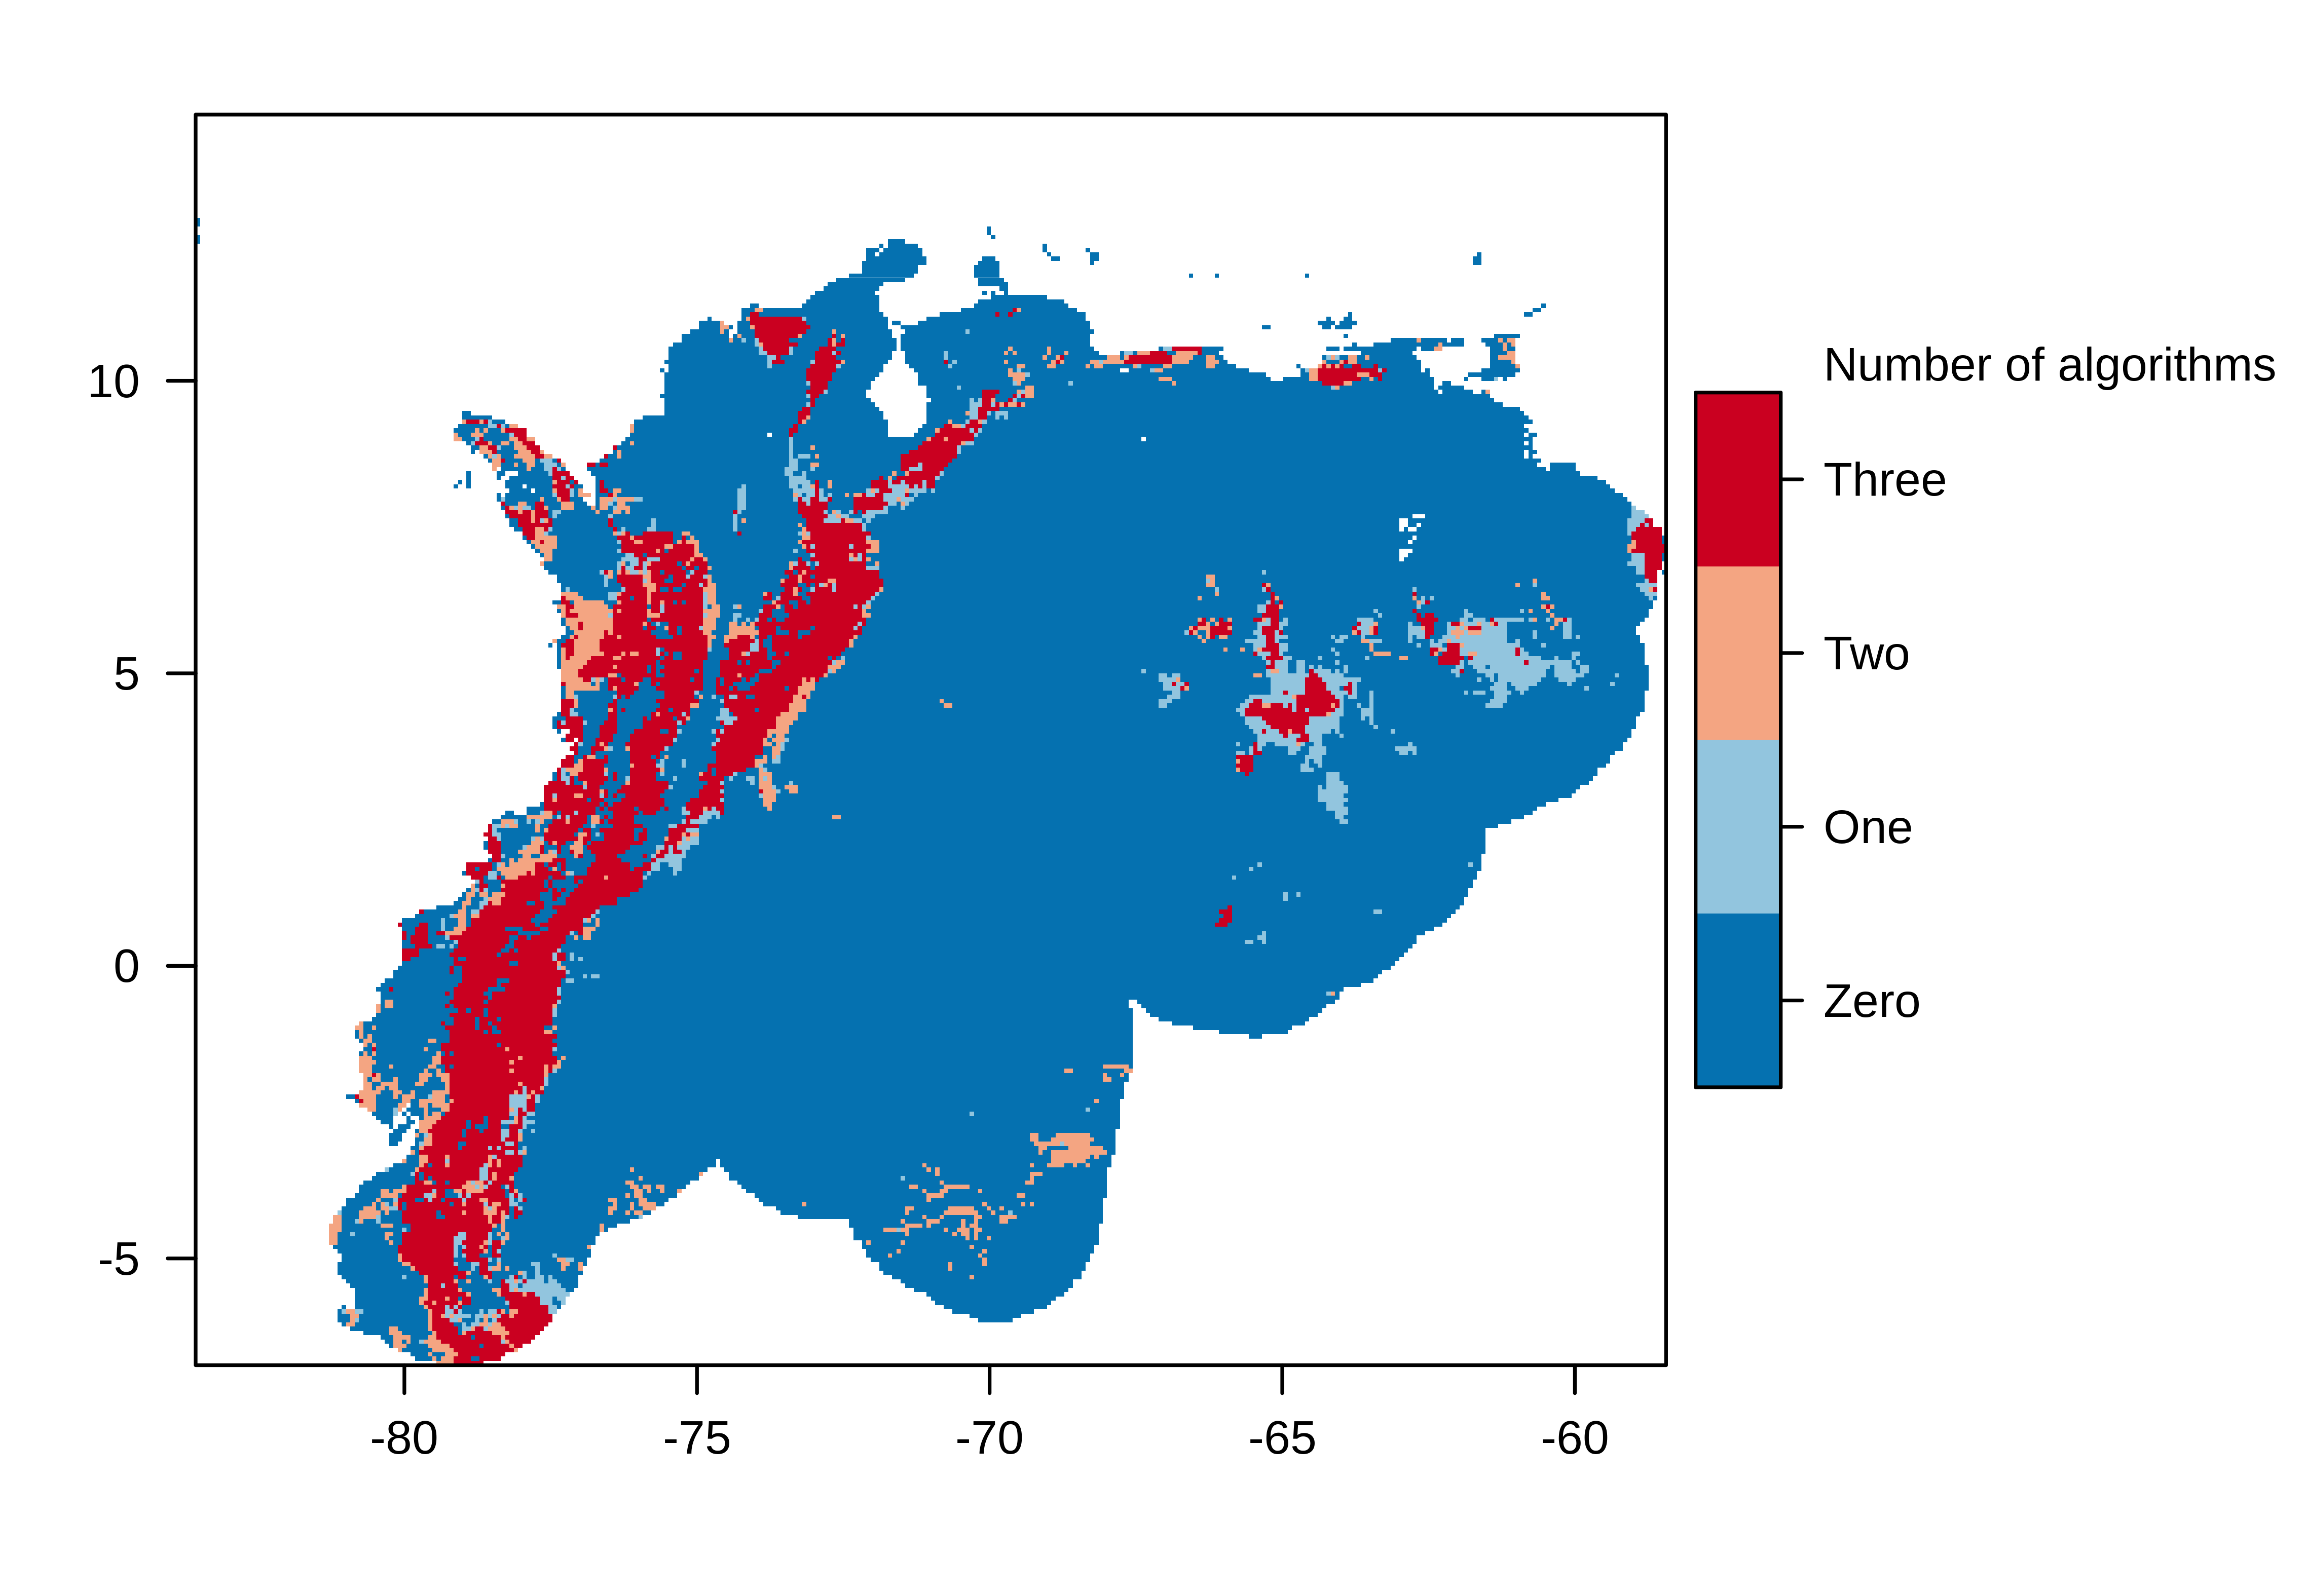
\includegraphics{NFPaper_files/figure-latex/unnamed-chunk-5-1.png}
In this example when we calculate the top 10\% of protected cells for Quadratic Network Flow we get 22,671 cells, 22,586 cells for linear Network Flow, and 22,671 cells for Zonation.

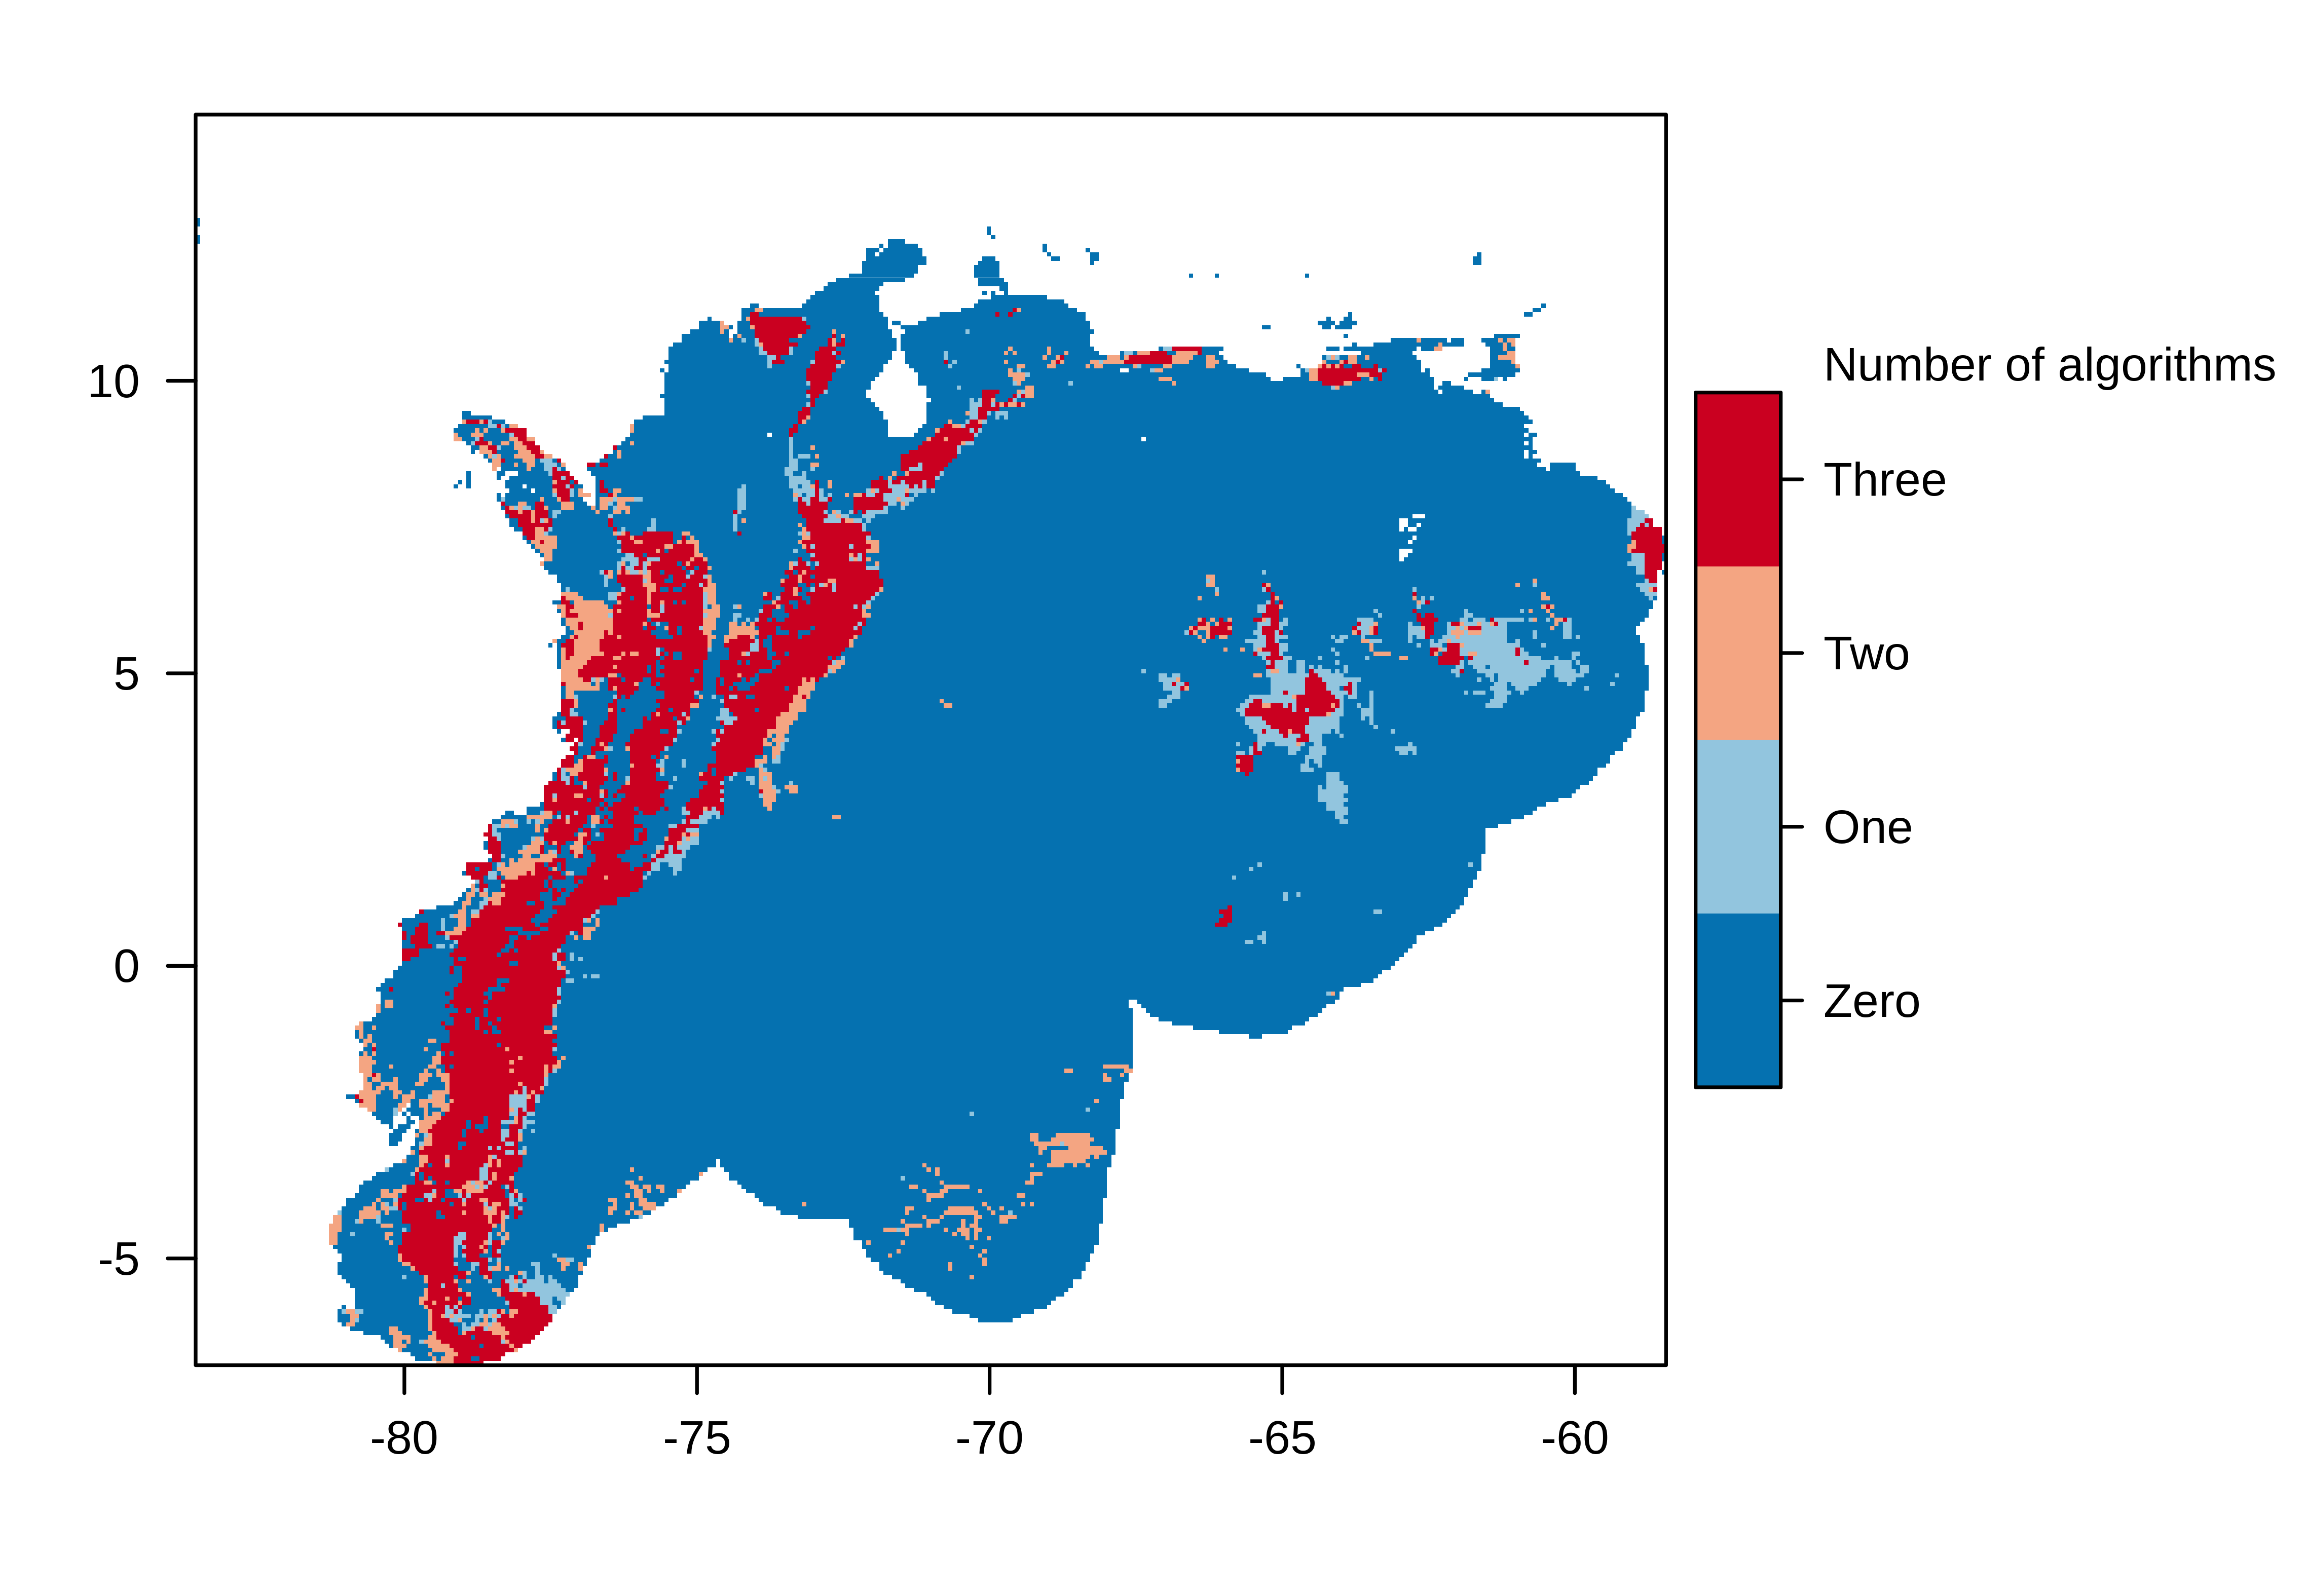
\includegraphics{NFPaper_files/figure-latex/unnamed-chunk-6-1.png}

\hypertarget{correlation-comparison-spearman}{%
\subsubsection{Correlation comparison (Spearman)}\label{correlation-comparison-spearman}}

\begin{table}[H]
\centering
\begin{tabular}{lrrr}
\toprule
rowname & Linear.NF & Quadratic.NF & Zonation\\
\midrule
Linear.NF & NA & 0.9211996 & 0.6241322\\
Quadratic.NF & 0.9211996 & NA & 0.6690281\\
Zonation & 0.6241322 & 0.6690281 & NA\\
\bottomrule
\end{tabular}
\end{table}

\begin{figure}
\centering
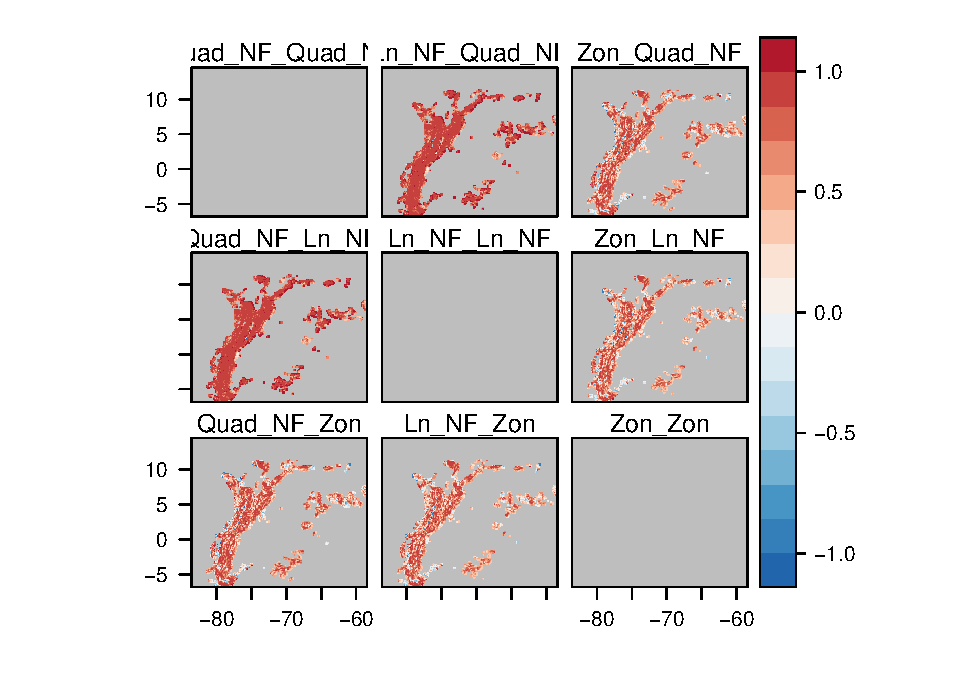
\includegraphics{NFPaper_files/figure-latex/LocalCorr-1.pdf}
\caption{\label{fig:LocalCorr}Box plot of local correlations between all three different methods of priorization}
\end{figure}

\begin{figure}
\centering
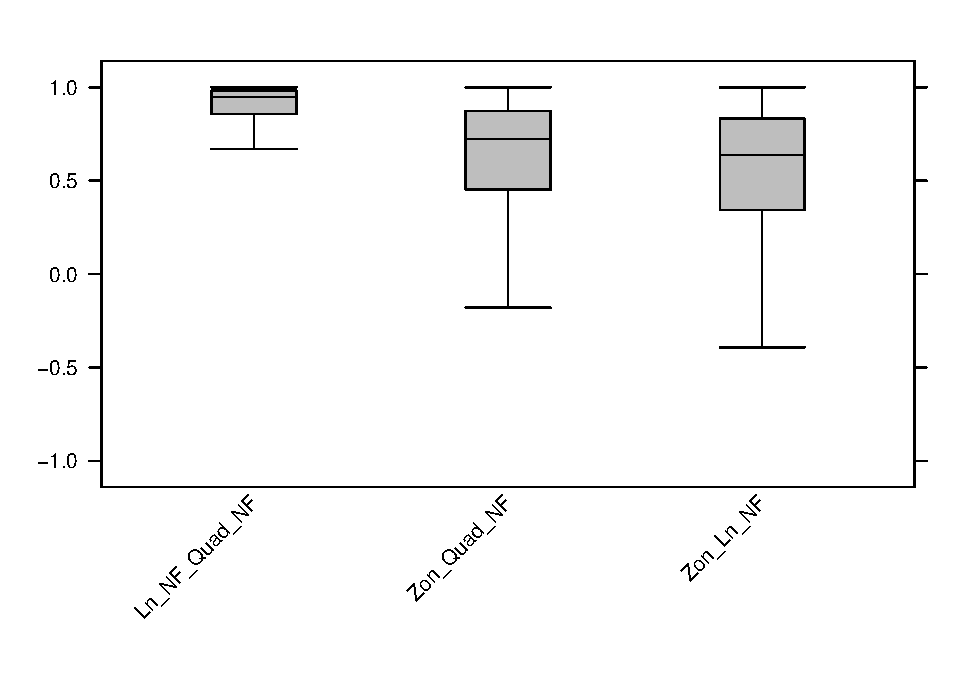
\includegraphics{NFPaper_files/figure-latex/Boxplot-1.pdf}
\caption{\label{fig:Boxplot}Box plot of local correlations between all three different methods of priorization}
\end{figure}

\hypertarget{discussion}{%
\section{Discussion}\label{discussion}}

\hypertarget{disclosureconflict-of-interest-statement}{%
\section*{Disclosure/Conflict-of-Interest Statement}\label{disclosureconflict-of-interest-statement}}
\addcontentsline{toc}{section}{Disclosure/Conflict-of-Interest Statement}

The authors declare that the research was conducted in the absence of any
commercial or financial relationships that could be construed as a potential
conflict of interest.

\hypertarget{author-contributions}{%
\section*{Author Contributions}\label{author-contributions}}
\addcontentsline{toc}{section}{Author Contributions}

The statement about the authors and contributors can be up to several sentences
long, describing the tasks of individual authors referred to by their initials
and should be included at the end of the manuscript before the References
section.

\hypertarget{acknowledgments}{%
\section*{Acknowledgments}\label{acknowledgments}}
\addcontentsline{toc}{section}{Acknowledgments}

Funding:

\hypertarget{supplemental-data}{%
\section{Supplemental Data}\label{supplemental-data}}

Supplementary Material should be uploaded separately on submission, if there are
Supplementary Figures, please include the caption in the same file as the
figure. LaTeX Supplementary Material templates can be found in the Frontiers
LaTeX folder

\hypertarget{references}{%
\section{References}\label{references}}

\hypertarget{figures}{%
\section*{Figures}\label{figures}}
\addcontentsline{toc}{section}{Figures}

\hypertarget{suplmentary-materials}{%
\section{Suplmentary materials}\label{suplmentary-materials}}

\hypertarget{list-of-species}{%
\subsection{List of species}\label{list-of-species}}

The species used for the solution were the folowing:

Aa maderoi, Abutilon ibarrense, Achyrocline crassiceps, Aciachne flagellifera, Aechmea drakeana, Aegiphila pennellii, Aequatorium sinuatifolium, Aequatorium verrucosum, Aetheolaena involucrata, Aetheolaena lingulata, Ageratina asclepiadea, Ageratina dendroides, Ageratina gynoxoides, Ageratina pseudochilca, Ageratina theaefolia, Ageratina vacciniaefolia, Agouticarpa grandistipula, Agrostis boyacensis, Agrostis foliata, Agrostis trichodes, Aiphanes grandis, Altensteinia virescens, Amazilia castaneiventris, Anagallis foemina, Anastrophyllum nigrescens, Andigena laminirostris, Anomobryum prostratum, Anotomys leander, Anredera brachystachys, Anthopterus schultzeae, Anthurium aristatum, Anthurium carchiense, Anthurium cordiforme, Anthurium flavolineatum, Anthurium giganteum, Anthurium gualeanum, Anthurium herthae, Anthurium lancea, Anthurium membranaceum, Anthurium morae, Anthurium palenquense, Anthurium pallatangense, Anthurium pedunculare, Anthurium pendulispadix, Anthurium phyllobaris, Anthurium rimbachii, Anthurium rugulosum, Anthurium wattii, Aphanactis jamesoniana, Aphanactis ollgaardii, Aphanactis piloselloides, Aragoa abietina, Aragoa cundinamarcensis, Aragoa occidentalis, Arcytophyllum aristatum, Arenaria venezuelana, Aristeguietia glutinosa, Arracacia moschata, Arremon phaeopleurus, Astragalus geminiflorus, Astragalus sprucei, Atlapetes flaviceps, Atlapetes leucopis, Atractus crassicaudatus, Atractus lasallei, Axinaea merianiae, Axinaea sodiroi, Azorella aretioides, Azorella cuatrecasasii, Azorella pedunculata, Baccharis revoluta, Baccharis rupicola, Baccharis teindalensis, Badilloa salicina, Bangsia aureocincta, Bangsia edwardsi, Bangsia rothschildi, Bartsia laticrenata, Bartsia orthocarpiflora, Bartsia santolinifolia, Bartsia stricta, Bauhinia stenantha, Begonia tiliifolia, Belloa radians, Berberis goudotii, Berberis hallii, Berberis rigidifolia, Berberis verticillata, Besleria angustiflora, Blakea glandulosa, Blakea hispida, Blakea oldemanii, Blakea rotundifolia, Bolborhynchus ferrugineifrons, Bomarea glaucescens, Bomarea linifolia, Bomarea patacocensis, Bomarea uncifolia, Brachtia andina, Brachyotum alpinum, Brachyotum confertum, Brachyotum fictum, Brachyotum gleasonii, Brachyotum harlingii, Brachyotum jamesonii, Brachyotum strigosum, Brayopsis colombiana, Breutelia squarrosa, Breutelia trianae, Browneopsis disepala, Brugmansia aurea, Brunellia boqueronensis, Brunellia colombiana, Bucquetia glutinosa, Buddleja pichinchensis, Burmeistera montipomum, Calamagrostis aurea, Calamagrostis effusa, Calamagrostis fibrovaginata, Calamagrostis guamanensis, Calamagrostis mollis, Calamagrostis podophora, Calceolaria dilatata, Calceolaria ferruginea, Calceolaria hyssopifolia, Calceolaria lamiifolia, Calceolaria pedunculata, Calceolaria purpurascens, Calceolaria rosmarinifolia, Calliergonella cuspidata, Campylopus argyrocaulon, Campylopus cleefii, Campylopus cucullatifolius, Campylopus edithae, Campylopus incertus, Campylopus pittieri, Campylopus subconcolor, Carex amicta, Casearia mexiae, Castilleja nubigena, Castratella piloselloides, Centradeniastrum album, Centropogon aequatorialis, Centropogon baezanus, Centropogon glabrifilis, Centropogon medusa, Centropogon nigricans, Centropogon subandinus, Cerastium floccosum, Ceratostema alatum, Cestrum peruvianum, Chalcostigma heteropogon, Chorisodontium speciosum, Chromolaena bullata, Chusquea subulata, Cinclodes excelsior, Cistothorus apolinari, Cistothorus meridae, Citharexylum sulcatum, Clavija eggersiana, Clethra crispa, Clinopodium nubigenum, Clinopodium taxifolium, Clinopodium tomentosum, Clusia callejasii, Coespeletia moritziana, Coespeletia spicata, Coespeletia thyrsiformis, Coespeletia timotensis, Colignonia pentoptera, Columnea albiflora, Columnea capillosa, Columnea ciliata, Columnea eubracteata, Conirostrum rufum, Conyza cardaminifolia, Conyza trihecatactis, Coursetia gracilis, Coussarea pilosiflora, Cranichis antioquiensis, Cranioleuca hellmayri, Critoniopsis occidentalis, Critoniopsis palaciosii, Critoniopsis sodiroi, Cronquistianthus niveus, Croton elegans, Croton rimbachii, Cryptotis equatoris, Culcitium nivale, Cyanolyca pulchra, Cynanchum microphyllum, Dalea humifusa, Dasyphyllum popayanense, Dendrophorbium lloense, Diglossa gloriosa, Diglossa gloriosissima, Diglossa indigotica, Diplostephium alveolatum, Diplostephium bicolor, Diplostephium cayambense, Diplostephium cinerascens, Diplostephium ericoides, Diplostephium frontinense, Diplostephium glandulosum, Diplostephium hartwegii, Diplostephium ochraceum, Diplostephium phylicoides, Diplostephium revolutum, Diplostephium rhododendroides, Diplostephium rhomboidale, Diplostephium rupestre, Diplostephium schultzii, Diplostephium spinulosum, Diplostephium tenuifolium, Diplostephium tolimense, Diplostephium violaceum, Diplostichum longirostre, Distichia acicularis, Ditrichum submersum, Draba aretioides, Draba hallii, Draba obovata, Draba splendens, Draba spruceana, Dracula sodiroi, Drepanocladus exannulatus, Drymonia crenatiloba, Drymonia laciniosa, Dysithamnus occidentalis, Elaphoglossum antisanae, Elaphoglossum heliconiifolium, Elaphoglossum yatesii, Elasis hirsuta, Elatine ecuadoriensis, Elleanthus gastroglottis, Elleanthus petrogeiton, Epidendrum englerianum, Epidendrum marsupiale, Epidendrum pallatangae, Epidendrum pichinchae, Epidendrum porphyreum, Eragrostis condensata, Erigeron ecuadoriensis, Eriocnemis cupreoventris, Eriocnemis derbyi, Eriocnemis mosquera, Eryngium humboldtii, Espeletia argentea, Espeletia barclayana, Espeletia batata, Espeletia boyacensis, Espeletia brassicoidea, Espeletia cleefii, Espeletia congestiflora, Espeletia conglomerata, Espeletia frontinoensis, Espeletia grandiflora, Espeletia hartwegiana, Espeletia killipii, Espeletia lopezii, Espeletia murilloi, Espeletia pycnophylla, Espeletia schultesiana, Espeletia schultzii, Espeletia semiglobulata, Espeletia summapacis, Espeletia tunjana, Espeletia uribei, Espeletiopsis colombiana, Espeletiopsis corymbosa, Espeletiopsis pannosa, Espeletiopsis petiolata, Eudema nubigena, Euphonia concinna, Festuca andicola, Festuca chimborazensis, Festuca glumosa, Festuca subulifolia, Festuca vaginalis, Fuchsia ampliata, Fuchsia caucana, Fuchsia dependens, Fuchsia hartwegii, Fuchsia macrostigma, Fuchsia orientalis, Fuchsia sessilifolia, Fuchsia sylvatica, Fuchsia vulcanica, Gasteranthus columbianus, Gasteranthus lateralis, Gasteranthus leopardus, Gasteranthus quitensis, Gaultheria cordifolia, Geissanthus argutus, Genista monspessulana, Gentianella cerastioides, Gentianella cernua, Gentianella corymbosa, Gentianella foliosa, Gentianella hirculus, Gentianella hyssopifolia, Gentianella nummulariifolia, Gentianella rapunculoides, Gentianella rupicola, Geonoma divisa, Geranium maniculatum, Geranium multiceps, Geranium multipartitum, Glaucidium nubicola, Gongylolepis jauaensis, Grallaria alleni, Grallaria flavotincta, Grallaria milleri, Grallaria rufocinerea, Grallaricula lineifrons, Grallaricula loricata, Grosvenoria hypargyra, Grosvenoria rimbachii, Gustavia longifuniculata, Gustavia serrata, Guzmania jaramilloi, Guzmania lehmanniana, Guzmania vanvolxemii, Guzmania wittmackii, Gynoxys acostae, Gynoxys hirsuta, Gynoxys laurata, Gynoxys miniphylla, Gynoxys parvifolia, Gynoxys pendula, Gynoxys sodiroi, Gynoxys stuebelii, Gynoxys tolimensis, Halenia adpressa, Halenia gentianoides, Halenia pulchella, Haplophaedia lugens, Hebeclinium tetragonum, Hedyosmum parvifolium, Heliangelus strophianus, Heliconia dielsiana, Heppiella verticillata, Hesperomeles goudotiana, Hieracium avilae, Huperzia capellae, Huperzia cruenta, Huperzia cumingii, Huperzia hystrix, Huperzia lindenii, Huperzia llanganatensis, Huperzia polydactyla, Huperzia rufescens, Huperzia transilla, Huperzia unguiculata, Hypericum decandrum, Hypericum goyanesii, Hypericum myricariifolium, Hypericum prostratum, Hypericum quitense, Hypochaeris setosa, Inga extra-nodis, Isoetes andina, Isoetes bischlerae, Isoetes boyacensis, Isoetes novo-granadensis, Isoetes palmeri, Jamesonia bogotensis, Jamesonia cinnamomea, Jamesonia pulchra, Juncus breviculmis, Juncus echinocephalus, Juncus ecuadoriensis, Lachemilla angustata, Lachemilla hirta, Lachemilla hispidula, Lachemilla holosericea, Lachemilla jamesonii, Lachemilla nivalis, Lachemilla rupestris, Lachemilla tanacetifolia, Lasiocephalus ovatus, Ledothamnus luteus, Lepanthes effusa, Lepanthes pilosella, Lepechinia vulcanicola, Lepidozia macrocolea, Leptodontium erythroneuron, Leptoscyphus cleefii, Leptotila conoveri, Liabum saloyense, Llerasia hypoleuca, Loricaria antisanensis, Loricaria complanata, Loricaria ilinissae, Lourteigia humilis, Lourteigia microphylla, Lupinus alopecuroides, Lupinus colombiensis, Lupinus smithianus, Lysipomia montioides, Lysipomia muscoides, Macleania bullata, Macleania coccoloboides, Macleania cordifolia, Macleania ericae, Macleania loeseneriana, Macrocarpaea glabra, Margarornis stellatus, Masdevallia ophioglossa, Matisia palenquiana, Mauritiella macroclada, Melothria longituba, Melpomene assurgens, Melpomene sodiroi, Meriania heptamera, Meriania hernandoi, Metallura baroni, Metallura williami, Mezobromelia lyman-smithii, Miconia aguirrei, Miconia biappendiculata, Miconia chlorocarpa, Miconia dielsii, Miconia glandulistyla, Miconia hymenanthera, Miconia nodosa, Miconia pernettifolia, Miconia pichinchensis, Miconia psychrophila, Miconia scutata, Miconia summa, Miconia turgida, Mimosa quitensis, Mimosa townsendii, Mona meridensis, Monnina crassifolia, Monnina equatoriensis, Monnina obtusifolia, Monnina pseudopilosa, Monnina revoluta, Monnina sodiroana, Monnina tenuifolia, Monticalia arbutifolia, Monticalia peruviana, Monticalia vaccinioides, Morella singularis, Muscisaxicola alpinus, Mutisia grandiflora, Mutisia microphylla, Mutisia sodiroi, Myioborus albifrons, Myrrhidendron glaucescens, Myrsine panamensis, Niphogeton azorelloides, Niphogeton glaucescens, Niphogeton josei, Notopleura marginata, Nototriche jamesonii, Nototriche phyllanthos, Odontoglossum hallii, Odontophorus atrifrons, Odontophorus melanonotus, Oncidium serratum, Opuntia soederstromiana, Oreobolus cleefii, Oreopanax corazonensis, Oreopanax ecuadorensis, Oreopanax ellsworthii, Oreopanax grandifolius, Oreopanax mutisianus, Oreopanax nigrum, Oreopanax palamophyllus, Oreopanax ruizanus, Oreothraupis arremonops, Oreotrochilus chimborazo, Ossaea sessilifolia, Oxypogon guerinii, Paepalanthus alpinus, Paepalanthus karstenii, Paepalanthus lodiculoides, Palicourea prodiga, Palicourea sodiroi, Palicourea subalatoides, Pappobolus imbaburensis, Paspalum hirtum, Passiflora adulterina, Passiflora crispolanata, Passiflora cuatrecasasii, Passiflora jamesonii, Passiflora roseorum, Passiflora trinervia, Pedicularis incurva, Pentacalia abietina, Pentacalia americana, Pentacalia arbutifolia, Pentacalia flosfragrans, Pentacalia guadalupe, Pentacalia ledifolia, Pentacalia nitida, Pentacalia pulchella, Pentacalia reissiana, Pentacalia vaccinioides, Pentacalia vernicosa, Pentagonia grandiflora, Peperomia fuscipunctata, Peperomia miqueliana, Pernettya hirta, Phalcoboenus carunculatus, Philodendron oligospermum, Philodendron rugosum, Philonotis andina, Pilea gallowayana, Pinguicula elongata, Piper laguna-cochanum, Piper sodiroi, Piper subflavum, Pipreola jucunda, Pitcairnia commixta, Pitcairnia cosangaensis, Pitcairnia fusca, Pittosporum undulatum, Plagiocheilus frigidus, Plagiocheilus solivaeformis, Pleurothallis ensata, Pleurothallis macra, Pleurothallis truncata, Plutarchia guascensis, Poa cucullata, Poa paramoensis, Poa pauciflora, Polylepis lanuginosa, Polylepis quadrijuga, Polylepis reticulata, Polypodium mindense, Polypodium monosorum, Polypodium segregatum, Polytrichadelphus ciliatus, Pouteria capacifolia, Prunus antioquensis, Prunus herthae, Psammisia debilis, Psammisia occidentalis, Psammisia sclerantha, Psychotria boqueronensis, Psychotria cuatrecasasii, Puya glomerifera, Puya goudotiana, Puya nitida, Puya santosii, Puya trianae, Pyrrhura hoematotis, Racinaea subalata, Rallus semiplumbeus, Ranunculus nubigenus, Renealmia fragilis, Renealmia sessilifolia, Rhodospatha densinervia, Rhodostemonodaphne laxa, Rhynchospora paramora, Ribes hirtum, Ribes lehmannii, Rubus choachiensis, Rubus gachetensis, Ruilopezia atropurpurea, Ruilopezia marcescens, Rumex tolimensis, Saguinus leucopus, Salvia pichinchensis, Saurauia chiliantha, Saurauia crassisepala, Saurauia omichlophila, Saurauia peduncularis, Saurauia pseudostrigillosa, Schefflera acaropunctata, Schefflera lasiogyne, Schefflera marginata, Schefflera ramosissima, Scorpidium scorpioides, Scytalopus griseicollis, Scytalopus rodriguezi, Scytalopus vicinior, Senecio culcitioides, Senecio formosoides, Senecio hypsobates, Senecio leucanthemoides, Senecio madagascariensis, Senecio niveoaureus, Senecio subruncinatus, Setaria cernua, Siparuna croatii, Siparuna palenquensis, Siphocampylus affinis, Siphocampylus brevicalyx, Siphocampylus columnae, Solanum crinitipes, Solanum paucijugum, Sorocea sarcocarpa, Sparrmannia africana, Sphaeradenia hamata, Sphaeradenia horrida, Sphagnum compactum, Sphagnum oxyphyllum, Sphyrospermum boekei, Sphyrospermum grandifolium, Sporobolus bogotensis, Stachys bogotensis, Stachys elliptica, Stelis columnaris, Stelis piperina, Stellaria recurvata, Stenospermation longifolium, Stilpnophyllum grandifolium, Stilpnophyllum oellgaardii, Stipa milleana, Stipa rosea, Symphyogyna bogotensis, Symplocos cundinamarcensis, Symplocos rhomboidea, Symplocos theiformis, Synallaxis castanea, Synallaxis subpudica, Syntrichia andicola, Tagetes zypaquirensis, Tangara rufigenis, Telipogon nervosus, Ternstroemia cleistogama, Terpsichore heteromorpha, Terpsichore pichinchae, Tetragastris varians, Thelypteris rigescens, Themistoclesia epiphytica, Theobroma gileri, Thibaudia andrei, Thibaudia grantii, Thibaudia parvifolia, Thomasomys hylophilus, Thomasomys niveipes, Thryophilus nicefori, Tibouchina gleasoniana, Tibouchina paleacea, Tibouchina pendula, Tillandsia emergens, Tillandsia incarnata, Tillandsia lajensis, Tillandsia secunda, Tillandsia superba, Tillandsia truncata, Tournefortia ramosissima, Uncinia paludosa, Uniola condensata, Urothraupis stolzmanni, Urtica longispica, Valeriana adscendens, Valeriana arborea, Valeriana bracteata, Valeriana tatamana, Valeriana tomentosa, Verbesina brachypoda, Verbesina latisquama, Verbesina lloensis, Verbesina sodiroi, Viburnum anabaptista, Viburnum antioquiense, Vigna venusta, Viola glandularis, Vireo masteri, Weinmannia polyphylla, Wettinia anomala, Xenophyllum crassum, Zanthoxylum lepidopteriphilum, Zygodon pichinchensis

--\textgreater{}

--\textgreater{}

--\textgreater{}

--\textgreater{}

--\textgreater{}

--\textgreater{}

--\textgreater{}

--\textgreater{}

--\textgreater{}

--\textgreater{}
 --\textgreater{}
 --\textgreater{}
 --\textgreater{}
 --\textgreater{}
 --\textgreater{}

--\textgreater{}

--\textgreater{}

--\textgreater{}
 --\textgreater{}
 --\textgreater{}
 --\textgreater{}
 --\textgreater{}

--\textgreater{}

--\textgreater{}

--\textgreater{}

--\textgreater{}

--\textgreater{}

--\textgreater{}

\hypertarget{refs}{}
\leavevmode\hypertarget{ref-Ahuja93}{}%
Ahuja, Ravindra K., Thomas L. Magnanti, and James B. Orlin. 1993. \emph{Network Flows: Theory, Algorithms, and Applications}. Englewood Cliffs, NJ: Prentice Hall.

\leavevmode\hypertarget{ref-alagador2014shifting}{}%
Alagador, Diogo, Jorge Orestes Cerdeira, and Miguel Bastos Araújo. 2014. ``Shifting Protected Areas: Scheduling Spatial Priorities Under Climate Change.'' \emph{Journal of Applied Ecology} 51 (3). Wiley Online Library: 703--13.

\leavevmode\hypertarget{ref-araujo2004would}{}%
Araújo, Miguel B, Mar Cabeza, Wilfried Thuiller, Lee Hannah, and Paul H Williams. 2004. ``Would Climate Change Drive Species Out of Reserves? An Assessment of Existing Reserve-Selection Methods.'' \emph{Global Change Biology} 10 (9). Wiley Online Library: 1618--26.

\leavevmode\hypertarget{ref-beier2007linkage}{}%
Beier, P, DR Majka, and T Bayless. 2007. ``Linkage Designs for Arizona's Missing Linkages.'' \emph{Arizona Game and Fish Department, Phoenix}.

\leavevmode\hypertarget{ref-chen2011rapid}{}%
Chen, I-Ching, Jane K Hill, Ralf Ohlemüller, David B Roy, and Chris D Thomas. 2011. ``Rapid Range Shifts of Species Associated with High Levels of Climate Warming.'' \emph{Science} 333 (6045). American Association for the Advancement of Science: 1024--6.

\leavevmode\hypertarget{ref-Corcoran_Quadcost}{}%
Corcoran, Derek, and Javier Fajardo. 2019. \emph{QuadCostAmpl: Transforms a Stack of Timeslices of Species Distribution Models into Data for Ampl Modeling}. \url{https://github.com/derek-corcoran-barrios/QuadCostAmpl}.

\leavevmode\hypertarget{ref-cushman2013biological}{}%
Cushman, Samuel A, Brad McRae, Frank Adriaensen, Paul Beier, Mark Shirley, and Kathy Zeller. 2013. ``Biological Corridors and Connectivity {[}Chapter 21{]}.'' \emph{In: Macdonald, DW; Willis, KJ, Eds. Key Topics in Conservation Biology 2. Hoboken, NJ: Wiley-Blackwell. P. 384-404.} Wiley Online Library, 384--404.

\leavevmode\hypertarget{ref-di2014quick}{}%
Di Minin, Enrico, Victoria Veach, Joona Lehtomäki, Federico Montesino Pouzols, Atte Moilanen, and others. 2014. ``A Quick Introduction to Zonation.'' Helsingin yliopisto.

\leavevmode\hypertarget{ref-fajardo_javier_2018_2669407}{}%
Fajardo, Javier, Derek Corcoran, Patrick Roehrdanz, Lee Hannah, and Pablo Marquet. 2018. \url{https://doi.org/10.5281/zenodo.2669407}.

\leavevmode\hypertarget{ref-gregory2014forecasts}{}%
Gregory, Stephen D, Marc Ancrenaz, Barry W Brook, Benoit Goossens, Raymond Alfred, Laurentius N Ambu, and Damien A Fordham. 2014. ``Forecasts of Habitat Suitability Improve Habitat Corridor Efficacy in Rapidly Changing Environments.'' \emph{Diversity and Distributions} 20 (9). Wiley Online Library: 1044--57.

\leavevmode\hypertarget{ref-hannah2007protected}{}%
Hannah, Lee, Guy Midgley, Sandy Andelman, Miguel Araújo, Greg Hughes, Enrique Martinez-Meyer, Richard Pearson, and Paul Williams. 2007. ``Protected Area Needs in a Changing Climate.'' \emph{Frontiers in Ecology and the Environment} 5 (3). Wiley Online Library: 131--38.

\leavevmode\hypertarget{ref-Hanson2019}{}%
Hanson, Jeffrey O, Richard Schuster, Nina Morrell, Matthew Strimas-Mackey, Matthew E Watts, Peter Arcese, Joseph Bennett, and Hugh P Possingham. 2019. \emph{Prioritizr: Systematic Conservation Prioritization in R}. \url{https://CRAN.R-project.org/package=prioritizr}.

\leavevmode\hypertarget{ref-Hijmans_Dismo}{}%
Hijmans, Robert J., Steven Phillips, John Leathwick, and Jane Elith. 2017. \emph{Dismo: Species Distribution Modeling}. \url{https://CRAN.R-project.org/package=dismo}.

\leavevmode\hypertarget{ref-jenkins2015us}{}%
Jenkins, Clinton N, Kyle S Van Houtan, Stuart L Pimm, and Joseph O Sexton. 2015. ``US Protected Lands Mismatch Biodiversity Priorities.'' \emph{Proceedings of the National Academy of Sciences} 112 (16). National Acad Sciences: 5081--6.

\leavevmode\hypertarget{ref-jones2016incorporating}{}%
Jones, Kendall R, James EM Watson, Hugh P Possingham, and Carissa J Klein. 2016. ``Incorporating Climate Change into Spatial Conservation Prioritisation: A Review.'' \emph{Biological Conservation} 194. Elsevier: 121--30.

\leavevmode\hypertarget{ref-lawler2013projected}{}%
Lawler, JJ, AS Ruesch, JD Olden, and BH McRae. 2013. ``Projected Climate-Driven Faunal Movement Routes.'' \emph{Ecology Letters} 16 (8). Wiley Online Library: 1014--22.

\leavevmode\hypertarget{ref-lenoir2008significant}{}%
Lenoir, Jonathan, Jean-Claude Gégout, PA Marquet, P De Ruffray, and H Brisse. 2008. ``A Significant Upward Shift in Plant Species Optimum Elevation During the 20th Century.'' \emph{Science} 320 (5884). American Association for the Advancement of Science: 1768--71.

\leavevmode\hypertarget{ref-merow2013practical}{}%
Merow, Cory, Matthew J Smith, and John A Silander Jr. 2013. ``A Practical Guide to Maxent for Modeling Species' Distributions: What It Does, and Why Inputs and Settings Matter.'' \emph{Ecography} 36 (10). Wiley Online Library: 1058--69.

\leavevmode\hypertarget{ref-nunez2013connectivity}{}%
Nuñez, Tristan A, Joshua J Lawler, Brad H McRae, D John Pierce, Meade B Krosby, Darren M Kavanagh, Peter H Singleton, and Joshua J Tewksbury. 2013. ``Connectivity Planning to Address Climate Change.'' \emph{Conservation Biology} 27 (2). Wiley Online Library: 407--16.

\leavevmode\hypertarget{ref-phillips2006maximum}{}%
Phillips, Steven J, Robert P Anderson, and Robert E Schapire. 2006. ``Maximum Entropy Modeling of Species Geographic Distributions.'' \emph{Ecological Modelling} 190 (3-4). Elsevier: 231--59.

\leavevmode\hypertarget{ref-phillips2008optimizing}{}%
Phillips, Steven J, Paul Williams, Guy Midgley, and Aaron Archer. 2008. ``Optimizing Dispersal Corridors for the Cape Proteaceae Using Network Flow.'' \emph{Ecological Applications} 18 (5). Wiley Online Library: 1200--1211.

\leavevmode\hypertarget{ref-regos2016predicting}{}%
Regos, Adrián, Manuela D'Amen, Nicolas Titeux, Sergi Herrando, Antoine Guisan, and Lluı's Brotons. 2016. ``Predicting the Future Effectiveness of Protected Areas for Bird Conservation in Mediterranean Ecosystems Under Climate Change and Novel Fire Regime Scenarios.'' \emph{Diversity and Distributions} 22 (1). Wiley Online Library: 83--96.

\leavevmode\hypertarget{ref-rodrigues2004effectiveness}{}%
Rodrigues, Ana SL, Sandy J Andelman, Mohamed I Bakarr, Luigi Boitani, Thomas M Brooks, Richard M Cowling, Lincoln DC Fishpool, et al. 2004. ``Effectiveness of the Global Protected Area Network in Representing Species Diversity.'' \emph{Nature} 428 (6983). Nature Publishing Group: 640.

\leavevmode\hypertarget{ref-rosenberg1997biological}{}%
Rosenberg, Daniel K, Barry R Noon, and E Charles Meslow. 1997. ``Biological Corridors: Form, Function, and Efficacy.'' \emph{BioScience} 47 (10). JSTOR: 677--87.

\leavevmode\hypertarget{ref-unep2018ngs}{}%
UNEP-WCMC, IUCN. 2018. ``NGS (2018).'' \emph{Protected Planet Report}.

\leavevmode\hypertarget{ref-williams2005planning}{}%
Williams, Paul, Lee Hannah, Sandy Andelman, Guy Midgley, Miguel Araújo, Greg Hughes, Lisa Manne, Enrique Martinez-Meyer, and Richard Pearson. 2005. ``Planning for Climate Change: Identifying Minimum-Dispersal Corridors for the Cape Proteaceae.'' \emph{Conservation Biology} 19 (4). Wiley Online Library: 1063--74.

\leavevmode\hypertarget{ref-zappa2017storylines}{}%
Zappa, Giuseppe, and Theodore G Shepherd. 2017. ``Storylines of Atmospheric Circulation Change for European Regional Climate Impact Assessment.'' \emph{Journal of Climate} 30 (16): 6561--77.


\end{document}
